\documentclass{llncs}

\usepackage[bookmarks,bookmarksopen,bookmarksdepth=2]{hyperref} %sections as bookmarks in adobe pdf
\hypersetup{pdfpagemode=UseNone}
\usepackage{times}

\usepackage[english]{babel} 
\usepackage[utf8]{inputenc}  %% les accents dans le fichier.tex
\usepackage[T1]{fontenc}       %% Pour la c{\'e}sure des mots accentu{\'e}s
\usepackage{microtype} % optional, for aesthetics
\usepackage{tabularx} % nice to have
\usepackage{booktabs} % necessary for style

% For URLs in the references
\usepackage{url}
\usepackage{hyperref}
%\usepackage{verbatim}

% Advanced Math
%\usepackage{amsmath}
%\usepackage{amssymb}	% double line font letters (for number sets N,Z,D,Q,R)

% Images and Floats
\usepackage{epsfig}
%\usepackage{epstopdf}

%\usepackage{caption}
%\usepackage{subcaption}
%\usepackage{lscape}			% landscape
%\usepackage{array}			% align vertically in tables
%\usepackage{multirow}
%\usepackage{rotating}

% Theorems, Definitions, ... (always after 'amsmath')
%\usepackage{amsthm}
%\theoremstyle{definition}
%\newtheorem{prop}{Property}%[section]
%\newtheorem{defn}{Definition}%[section]

% Algorithm environment
%\usepackage{algorithm}
%\usepackage{algorithmic}

% Commutative diagrams
%\usepackage{diagrams}

%\usepackage{enumitem}

%\usepackage{listings}

% Put edit comments in a really ugly standout display

\usepackage{ifthen}
\usepackage{amssymb}
\usepackage[dvipsnames]{xcolor}
\newboolean{showcomments}
\setboolean{showcomments}{true} % toggle to show or hide comments
\ifthenelse{\boolean{showcomments}}
{\newcommand{\nb}[2]{
        \fcolorbox{gray}{yellow}{\bfseries\sffamily\scriptsize#1}
        {$\blacktriangleright$#2$\blacktriangleleft$}
    }
    \newcommand{\version}{\emph{\scriptsize$-$working$-$}}
}
{\newcommand{\nb}[2]{}
    \newcommand{\version}{}
}
\newcommand{\textunderscript}[1]{$_{\text{#1}}$}

\definecolor{ao}{rgb}{0.0, 0.5, 0.0}
\newcommand\es[1]{\nb{ES}{\textcolor{red}{\textsl{#1}}}}
\newcommand\mw[1]{\nb{MW}{\textcolor{blue}{\textsl{#1}}}}
\newcommand\rb[1]{\nb{RB}{\textcolor{ao}{\textsl{#1}}}}

%%%%%%%%%%%%%%%%%%%%%%%%%%%%%%%%%%%%%%%%%%%%%

% Standard shortcuts
\newcommand{\eg}{e.g.,~}										% exempli gratia (for the sake of example)
\newcommand{\ie}{i.e.,~}										% id est (that is)
\newcommand{\etal}{~et al.}									% et alia (and others)
\newcommand{\Fig}[1]{Fig.~\ref{#1}}  			% choose Fig. or Figure, depending on the style
\newcommand{\Table}[1]{Table~\ref{#1}}	    % Table reference
\newcommand{\Sect}[1]{Section~\ref{#1}}	  	% section name always with a capital S
\newcommand{\Model}[1]{\textsf{\small{#1}}} % name of any modeling artifact (e.g., formalism, model element, rule, ...)
\newcommand{\Code}[1]{\texttt{\small{#1}}}	% inline code
\providecommand{\e}[1]{\ensuremath{\times 10^{#1}}}	% scientific notation: x.10^y

%%%%%%%%%%%%%%%%%%%%%%%%%%%%%%%%%%%%%%%%%%%%%


\begin{document}
    
\title{Domain-Specific Model Distance Measures}

\author{Manuel Wimmer\inst{1} \and Eugene Syriani\inst{2} \and Robert Bill\inst{3}}
\institute{
    Johannes Kelper Universit{\"a}t Linz, Austria
    \and 
    Universit{\'e} de Montr{\'e}al, Canada
    \and
    Technical University Vienna, Austria}

\maketitle

\begin{abstract}
A lot of research was invested in the last decade to develop differencing methods for models to identify the changes performed between two model versions.
A difference model captures these changes. However, less attention was paid to distance computations of model versions. While different versions of a model may have a similar amount of differences,
the distance to a base model may be drastically different. Therefore, we present in this paper distance metrics for models, a method to automatically generate tool support for computing domain-specific distance measures and show the benefits of distance measures over differences in searching for model evolution explanations. The results of running different experiments show...\es{todo}
\end{abstract}

\keywords{Model comparison, Model diffing, Model distances, Model evolution}

\section{INTRODUCTION}

The emergence of model-driven engineering (MDE)~\cite{Schmidt2006a} has increased the need for dedicated techniques for model management~\cite{Kolovos2013a}.
In particular, a lot of research was invested in the last decade to develop differencing methods to identify the changes performed between two model versions.
As surveyed in~\cite{StephanC13}, most algorithms aim at computing differences and representing them in the form of difference models which capture the changes between model versions.
Difference models are critical in MDE, being used for various model management tasks, such as metamodel/model co-evolution, versioning or synchronization~\cite{Ruscio2012,Demuth2016}.

While most work has been focusing on differences, less attention was paid to quantifying the distance between model versions.
Distances are useful in addition to differences for several reasons.
First, while different versions of a model may have the same amount of differences, their distance to the base model may be drastically different.
Second, distances can be an additional metric to consider the evolution paths of models to reach a certain setting.
the movement of attributes between different classes in a class diagram.
For example, suppose we have classes $A,B,C,$ and $D$ connected in sequence with associations.
If we move an attribute from $A$ to any other class, we always get the same difference: the attribute deleted from $A$ and added to one of the other classes. However, a distance metric could tell us \textit{``how far''} we have moved the attribute away from $A$, leading to a different distance measures depending in which class it has moved to.

In this work, we present the notion of distance metrics for models as an additional measurement of the difference between models.
Furthermore, we provide a method to derive distance metrics tailored to the domain-specific language (DSL) at hand.
We implemented a software library to automatically generate domain-specific model distance calculators, given the metamodel and the semantical change operators of the DSL.
We apply the distance metrics on the use case of searching for the explanation of model evolution in terms of domain-specific change operations.
Our results show that using distance metrics outperforms common difference models techniques.
%Finally, we discuss potential benefits and challenges of using domain-specific distance measures in comparison to model differences in searching for model evolution explanations in terms of domain-specific change operations. Specifically, the results of running different experiments show...

In Section 2, we overview the background of our approach and motivate our work with a running example for our use case.
In Section 3 we present how to compute the model distance metrics and how to derive them for a particular DSL.
In Section 4, we briefly outline our implementation and the use case for the following evaluation section.
In Section 5, we evaluate the application of these metrics on our use case.
We discuss related work in Section 6 and conclude in Section 7. 

\section{BACKGROUND}
This project uses MOMot to search for the sequence of application of model transformation rules that lead an input model M1 to a target model M2. As running example, we use the PacmanGame domain, with the rules specified in Henshin.


Search based approaches

MOMot - maybe mention MOMoT just in the evaluation section? 



Having the evolution recovery problem athand, we apply our search-based framework MOMoT~\cite{Fleck15,FleckTW16}, to find the Pareto-optimal module evolutions. MOMoT\footnote{MOMoT: \url{http://martin-fleck.github.io/momot}} is a task- and algorithm-agnostic approach that combines SBSE and MDE.
It has been developed in previous work~\cite{Fleck15} and builds upon Henshin\footnote{Henshin: \url{http://www.eclipse.org/henshin}}~\cite{Arendt10} to define model transformations and the MOEA framework\footnote{MOEA Framework: \url{http://www.moeaframework.org}} to provide optimization techniques. In MOMoT, DSLs (i.e., metamodels) are used to model the problem domain and create problem instances (i.e., models), while model transformations are used to manipulate those instances.
The orchestration of those model transformations, i.e., the order in which the transformation rules are applied and how those rules need to be configured, is derived by using different heuristic search algorithms which are guided by the effect the transformations have on the given objectives.
In order to apply MOMoT for the given problem, we need to specify the necessary input.
2 model versions, change operators defined as Henshin rules, and the objectives for the search.

Objectives are either based on diff metrics or on distance metrics. 


\section{DOMAIN-SPECIFIC MODEL DISTANCES}
\subsection{Running example}\label{sec:example}

\begin{figure}
    \centering
    \includegraphics[width=\linewidth]{images/pacman_example}
    \caption{The initial model M1 and two possible models resulting from applying different rules of the Pacman game}
    \label{fig:example}
\end{figure}
%
We rely on the running example of a simplified Pacman game, a well-known game where Pacman navigates through grid nodes searching for food to eat, while ghosts try to kill him.
We implemented a DSL to define game configurations, based on~\cite{Syriani2013a}.
\Fig{fig:example} illustrates two Pacman game models in the concrete syntax of the DSL\es{first use of acronym?}.
Pacman, food, and ghosts are placed on grid nodes with an \texttt{on} reference.
Grid nodes are connected by \texttt{left}, \texttt{right}, \texttt{up}, and \texttt{down} references to define the permissible navigation of Pacman and ghosts.
The concrete syntax represents references by topological alignment rather than arrows.
In M1, Pacman is on grid node 21 which has an \texttt{up} reference to grid node 11 and a \texttt{right} reference to grid node 22.
A score object keeps track of the points of every food Pacman eats.
The point for red food is 1 and for green food is 3.
We define the operational semantics of the DSL in terms of an inplace model transformation, implemented with graph transformation rules as in~\cite{Syriani2013a}.
One rule represents Pacman eating food on a grid node and updating the score.
Another represents the ghost killing Pacman when they are on the same grid node.
Four rules for Pacman and four others for the ghost represent moving in each direction to an adjacent grid node.\es{should we show one rule in Henshin?}
Although the rules should obey certain scheduling, \eg killing has priority over moving to end the game, in this work, we assume that the transformation is a graph grammar \ie any rule can be applied at any time during the execution of the transformation\es{do we need this assumption?}.

In this running example, we are interested in finding the minimal sequence of rule applications starting from the initial model leading to the target model.
Search-based techniques are very useful to solve this problem.
They explore all possibilities of the search-space by generating intermediate models as a result of applying the rules while optimizing the objective to get closer to the target model.
For example, a minimal rule sequence to go from M1 to M2 in \Fig{fig:example} is Pacman moves up once, then moves right three times, eating the food each time, while the ghost also moves left twice.
A minimal rule sequence from M1 to M3 is Pacman moves right, then up, then left, eating the food each time, while the ghost moves up once.

Detecting the rule sequence requires to compare models at every step.
\es{In current approaches? cite?}To compute the difference between M1 and M2, a generic model comparison tool, like EMFCompare, would report that three food objects are deleted, two \texttt{on} references (Pacman and ghost) are changed, and the attribute value of the score is modified.
This tool would report the same information when we compare M1 and M3.
However, a domain expert would immediately detect that the there is a clear difference betweem: 10 rules are needed to obtain M2 and 7 rules to obtain M3.
Furthermore, the score value hints to which type of food Pacman ate.
Thus, the information output by common model differencing approaches is not precise enough to identify the minimal sequence of rules (\eg for the M2 case, if Pacman moves right first, he will have to go through grid 12 node at least twice).
The main reason is that they rely solely on changes in the abstract syntax.
However, the comparison needs to be tailored to both the DSL and its semantics to find the best rule sequence.
In this example, relying on creation, deletion, and modification of elements of the metamodel is not sophisticated enough.
The notion of Pacman and ghost movements as well as a quantification of the score value must be encoded in the comparison.
Inplace model transformation rules typically encode semantic operations, such as operational semantics or refactoring~\cite{Lucio2016}.
Therefore, we propose a set of domain-specific distance metrics that take into consideration abstract syntax changes as well as the semantics of the transformation to provide more precise information when comparing models.
This would optimize the search space of identifying the minimal sequence of rule applications.
%
%\es{to be used where needed}\begin{itemize}
%    \item[Regular difference results:]
%        3 food objects deleted ;
%        2 on references modified ;
%        1 score value attribute modified.
%    
%    \item[Distance results:]
%        Move distance is $3+2=5$ ;
%        Value distance is $\frac{|4-1|}{4}=0.75$ ;
%        Element distance is $\frac{3+0}{13+10}=0.13$.
%    
%    \item[Minimal rules applied:]
%        1 Pacman Move Up ;
%        2 Pacman Move Right ;
%        3 Pacman Eats Food ;
%        2 Ghost Move Left.
%\end{itemize}

\subsection{Model distance metrics}

Typical model difference tools report metrics on elements added and deleted in terms of instances of metamodel classes, on references changed in terms of instances of metamodel associations, and on attribute value modifications.
For our purpose, we need metrics that are tailored to the DSL both in terms of the metamodel and the semantics of the transformation.
Therefore, we propose the following three model distance metrics.
These metrics are measured between two models M1 and M2, where M2 is the result of applying a sequence of rules on M1.

The semantics of many formalisms relies on movements of model elements.
Some of their elements are \emph{movable} while others represent \emph{positions} where an element can move to.
For example, Pacman moves on the grid in our example, attributes move to superclasses in class diagrams, or tokens move between places in a Petri net.
Furthermore, some elements are \emph{modifiable} meaning that the transformation changes some of their attribute values, like the score in the rule Pacman Eats Food.

Formally, we represent a model as a labeled, attributed multi-graph $G=\langle V,E,l,a \rangle$.
We identify three subsets of nodes $Mov,Pos,Mod \subset V$ corresponding to the movable, position, and modifiable objects.
In our running example, grid nodes are the position nodes and Pacman and ghosts are movable nodes.
Note that, in general, $Pos$ may be different for each $v \in Mov$.
Additionally, all three subsets need not to be disjoint nor complete: an object can move between positions, but it can also serve as a position for other movable objects, and it can have attributes modified.
Among the set of edges $e:V \rightarrow V \in E$, we identify two subsets $N,P \subset E$.
Neighbor edges $n: Pos \rightarrow Pos \in N$ only connect position nodes, \eg \texttt{left}, \texttt{right}, \texttt{up}, and \texttt{down} references between grid nodes.
Position edges $p: Mov \rightarrow Pos \in P$, like the \texttt{on} references, connect a movable node to a position node.
The label function $l:V \rightarrow \Sigma^*$ assigns a unique string label to each node.
The attribute function $a:V \times \Sigma^* \rightarrow \mathbb{N}$ assigns numerical values to each attribute name of a node.
%$w:Pos \rightarrow \mathbb{N}$ assigns numerical weight to each position edge.

\subsubsection{Move distance}
The move distance of a movable object is the length of the shortest path from its position in model M1 to its position in model M2.
We define $\delta_M(v_1,v_2)$ as the length of the shortest sequence of neighbor edges connecting $v_1$ to $v_2 \in Pos$.
In \Fig{fig:example}, $\delta_M(pacman,grid_{13})=3$ and $\delta_M(ghost,grid_{21})=2$, which is equivalent to the Manhattan distance in this grid layout.
To compute the move distance between M1 and M2, we identify the common connected subgraph $G_{12}$ of their respective graphs $G_1$ and $G_2$.
We define the move distance between two models as:
\[
\Delta_M(G_1,G_2)=\sum_{v_1,v_2 \in Mov_{12}}{\delta_M(p(v_1),p(v_2))} \mbox{, where } l(v_1)=l(v_2)
\]
Here, $p(v_1)$ is the position of $v_1$ in $G_1$ and $p(v_2)$ is its corresponding position in $G_2$.
In our example, $\Delta_M(M1,M2)=5$.
We rely on the popular Floyd-Warshall algorithm~\cite{Floyd1962,Warshall1962} to compute the shortest path between two nodes in a connected graph.
The dynamic programming implementation takes $O(|Pos|^3)$ to compute all distances between any two nodes and $O(|N|)$ to output the path.


\subsubsection{Element distance}
This metric is concerned with the presence and absence of metamodel class instances between M1 and M2.
This is similar to what a model difference algorithm outputs.
We define the element distance as:
\[
\Delta_E(G_1,G_2)=\frac{|\{v \in V_1 | \nexists v_2 \in V_2, l(v_2)=l(v)\}|+|\{v \in V_2 | \nexists v_1 \in V_1, l(v_1)=l(v)\}|}{|V_1|+|V_2|}
\]
The numerator counts the number of nodes exclusively in each graph.
To normalize the distance as a ratio between 0 and 1, we divide by the total number of nodes in both graphs.
In our example, $\Delta_E(M1,M2)=\frac{3+0}{13+10}=0.13$.
We can interpret this distance as the ratio of objects added or removed between the two models.
In this particular case, 13\% of the objects in M1 have been removed in M2.
Note that the element distance is not concerned with edges since they are already taken care of by the move distance.


\subsubsection{Value distance}
The third metric is concerned with the difference in attribute values between objects in M1 and M2.
We assume that any attribute value can be encoded as a unique number, a common practice for metrics~\cite{Bertoa2018}.
We define the value distance of attribute $x$ of node $v$ between $G_1$ and $G_2$ as:
\[
\delta_V(v,x)=\frac{|a(v,x)-a(v_1,x)|}{a(v,x)} \mbox{, where } v_1 \in Mod_1, v \in Mod_2 \mbox{ and } l(v)=l(v1)
\]
Here, we only consider attributes of objects present in both M1 and M2 because the element distance already takes care of the absence and presence of elements.
This distance computes the margin of error needed to obtain the value of $x$ in $v$ from its value in $v_1$.
We define the value distance $\Delta_V(G1,G2)$ between two models as the average of $\delta_V$ for all attributes of all nodes in $G_{12}$.
This calculates the average margin of error between all attribute values of the two models.
In our example, $\Delta_V(M1,M2)=\delta_V(score,value)=\frac{|4-1|}{4}=0.75$.

%
%\begin{itemize}
%	\item[Move distance:] There is often movement of elements (\eg pacman moving on the grid, attributes moving around classes). The move distance of a movable object is the length of the shortest path from its position in M1 to its position in M2. Move distance is related to computing the difference with Ecore references.
%	\item[Element distance:] Is the difference in the presence/absence of elements in M1 and M2. The element distance is the ratio, between 0 and 1, of the number of differences with respect to the total number of objects in M1 and M2.
%	\item[Value distance:] Is the difference in attribute values between M1 and M2. We assume that any attribute type can be encoded as numbers. Then the value distance of attribute x is its margin of error: $|M2.x - M1.x| / M2.x$. In this case, M2 acts as the expected target.
%	
%\end{itemize}
%
%The \emph{Move distance} relies on the Floyd-Marshall algorithm that computes the shortest from any position element to any position element in an Ecore model. This code is in EcoreShortestPaths and is independent from the domain. Its only external dependency is an interface IEReferenceNavigator which provides a function that gives the neighbor(s) of a position element. DistanceUtil provides all the necessary methods the move distance requires.
%
%The \emph{Value distance} is an average of all attribute distances. We only consider attributes of objects present in both M1 and M2 because the element distance takes care of absence and presence of elements. We assume that any attribute value can be represented as a unique number, which is common~\cite{Bertoa2018}. DistanceUtil provides the toDouble method to perform that conversion. Currently, it only supports number values encoded as Number or String data types. For each attribute, we compute its margin of error.
%
%The \emph{Element distance} looks for the objects present in M1 but not M2 and M2 but not M1. This is then divided by the size of M1 and M2. We only consider objects instances of metamodel classes. So references and attributes are not taken into account in this measure. This distance relies on the unique ID of each object as returned by the getId method.
%
%DistanceCalculator is the abstract class at the root that should be inherited by your distance function. For example MoveDistance only relies on the move distance between M1 and M2.

\subsection{Adapting distance metrics to the DSL}

The distance metrics presented in \Sect{sec:metrics} are generic model distances to compare two models.
We now describe how to adapt these metrics for a particular DSL and its semantics.
We aim to produce a distance calculator given the metamodel of the DSL and a set of inplace model transformation rules encoding its semantics.
Typically, these rules have a precondition and a postcondition pattern.

We need to identify the metamodel classes corresponding to the sets of nodes $Pos$ and $Mov$, and the associations corresponding to the sets of edges $N$ and $P$.
The potential candidates for $Mov$ are classes that have an association to another class in the metamodel with cardinality at most 1.
We denote $A$ the potentially movable class and $r$ its association to the other class $B$.
Instances of $A,r,$ and $B$ must be in the precondition of a rule and $r$ must be modified in the postcondition to reference another class instance.
Then, potentially $A$ is a class of movable nodes, $r$ is a position edge type, and $B$ is a class of position nodes.
In our example, these are, among others, the \texttt{Pacman} class, the \texttt{on} association, and the \texttt{GridNode} class, respectively.
It is also possible that $r$ is an association from $B$ to $A$.
Furthermore, it may be that the second instance $A$ refers to is of another type than $B$, say $C$.
If there is a reference $s$ between $B$ and $C$, then $s$ is likely to be a neighbor edge.
Note that this is a necessary condition but not sufficient.
For example, it may be the case where the movable and position classes are connected directly but through an intermediate class.

Similarly, we analyze the classes of the metamodel such that one of its attribute value is modified in the postcondition of a rule.
Such classes define the type of the nodes in $Mod$.

The three distance metrics rely on the label function $l$ to correspond similar nodes between the two models.
For example in \Fig{fig:example}, the grid nodes are identified by their identifier (\eg 11, 12, \ldots).
However, not all classes in the metamodel of the DSL have an identifying attribute.
Since the label function must uniquely identify each node, we must compute a label for each object that does not have one.
We can compute the label structurally.
For example, we can ascertain that there is at most one food on a grid node.
Then the label of a food object can rely on the label of the grid node it is on.
Another case is if we can ascertain that a class is a singleton, then we assign the same label to its instance.

From the above, we understand that automatically adapting the distance metrics to the DSL is very challenging.
Therefore, we implemented the distance metrics as a Java library that can compute the metrics on any Ecore model in the Eclipse Modeling Framework.
The library encapsulates all dependencies on the metamodel of the DSL within one abstract class \texttt{DistanceUtility}.
The developer must override the five sets $Pos,Mov,Mod,N,$ and $P$ for his DSL.
He must also define the \texttt{getId()} function for each class of the metamodel, if it does not already have an identity attribute.



%is movable if, when analyzing the rules, it has a reference to a position object and the rules modify that reference.
%Note that it could also be that a position object references a movable object.
%
%
%This implementation is just a proof of concept. It has been implemented with the mindset that the distance calculation is generated automatically from analyzing the metamodel and the transformation rules.
%
%Given a metamodel MM and Henshin rules R, we want to generate the distance calculator that will be used by the MOMot script.
%
%The domain-specific distance classes (e.g., the move, element, value distances) can be easily generated. They have two dependencies to the metamodel:
%
%The package instance, by overriding the getEPackageInstance() function
%The constructor, by instantiating the appropriate DistanceUtil singleton object specific to the metamodel
%
%Only the utility class (e.g., PacmanDistanceUtil) must be generated after analyzing MM and R. Following the code in PacmanDistanceUtil should guide you to know how to generate the code. Here are special considerations:
%
%Your Utility class must inherit from DistanceUtil.
%It should import all movable, position, modifiable, and other classes.
%It must provide a function used for its singleton instantiation as follows.
%
%It should have 4 attributes for movable, position, modifiable, and all other types.
%
%It should override all abstract methods from DistanceUtil.
%The tricky part is the generation of the Object getId(EObject object) method. If each object has attribute with setID(true) you can rely on super. Otherwise, you have to make up one unique on your own. For example, if you know for sure that an attribute is unique, then you can rely on it (e.g., Places and Transitions in the Petrinet example). If there is only one possible instance of this element, then return true (e.g., Scoreboard in the Pacman example). It can also rely on an object it references or that references it (e.g., Food in the Pacman example).
%
%You also need to generate the DistanceUtilFactory specific to the metamodel (e.g., PacmanGameDistanceUtilFactory). Its only purpose is to make the concrete DistanceUtil accessible as a singleton.
%
%\subsubsection{Customization}
%
%The only code that is specific to the metamodel is the class that implements DistanceUtil. This is where you define the functions that provide the following information:
%
%\begin{itemize}
%	\item[The movable objects:] An object is movable if, when analyzing the rules, it has a reference to a position object and the rules modify that reference. Note that it could also be that a position object references a movable object.
%	\item[The position objects:] An object is a position if, when analyzing the rules, it is what movable objects are always linked to. Note that it could also be that a position object references a movable object.
%	\item[The modifiable objects:] An object is modifiable if, when analyzing the rules, one of its attributes changes value.
%	\item[The other objects:] Any object that is not movable, position or modifiable.
%	\item[The ID of an object:] the value that uniquely identifies an object. This is used to find similar elements between M1 and M2.
%	\item[The modifiable attributes:] All attribute values subject to modification for a given object.
%	\item[Accessing the position:] the attribute used to know the position of a movable object.
%	\item[Accessing the neighbors of a position:] the attribute used to connect position objects.
%	\item[Accessing the root:] used to find the root object of M1 and M2.
%\end{itemize}

\section{EVALUATION AND DISCUSSION}
This project uses MOMot to search for the sequence of application of model transformation rules that lead an input model M1 to a target model M2. As running example, we use the PacmanGame domain, with the rules specified in Henshin.

Having the evolution recovery problem athand, we apply our search-based framework MOMoT~\cite{Fleck15,FleckTW16}, to find the Pareto-optimal module evolutions. MOMoT\footnote{MOMoT: \url{http://martin-fleck.github.io/momot}} is a task- and algorithm-agnostic approach that combines SBSE and MDE.
It has been developed in previous work~\cite{Fleck15} and builds upon Henshin\footnote{Henshin: \url{http://www.eclipse.org/henshin}}~\cite{Arendt10} to define model transformations and the MOEA framework\footnote{MOEA Framework: \url{http://www.moeaframework.org}} to provide optimization techniques. In MOMoT, DSLs (i.e., metamodels) are used to model the problem domain and create problem instances (i.e., models), while model transformations are used to manipulate those instances.
The orchestration of those model transformations, i.e., the order in which the transformation rules are applied and how those rules need to be configured, is derived by using different heuristic search algorithms which are guided by the effect the transformations have on the given objectives.
In order to apply MOMoT for the given problem, we need to specify the necessary input.
2 model versions, change operators defined as Henshin rules, and the objectives for the search.

Objectives are either based on diff metrics or on distance metrics.


Search based approaches

MOMot - maybe mention MOMoT just in the evaluation section?


 All experiments use the same input and output models, the same transformations, the same solution length and the 
same optimization algorithms and only differ in the fitness functions used in these algorithms. 
The exact Pacman and Petrinet cases have been freshly created for this evaluation, but are commonly used in the graph transformation world.
In the past, the Refactoring case has been used to evaluate different algorithms for MoMOT in the past, where all algorithms optimized the same fitness function. How, this case is used to evaluate the same algorithm with different fitness functions.


\subsection{Objective}

As our main goal is to compare different fitness functions in terms of their impact on search processes, we want to answer two research questions:

\begin{itemize}
	\item \textit{RQ1 - Search Space Exploration}: Is there a significant difference in the solutions found by applying each fitness function?
	\item \textit{RQ2 - Search Time}: Is there a significant difference in the number of iterations required to get good solutions?
	%Senseless - you can easily define simple generic model distance functions which are much faster, e.g. by just mapping things to feature vectors
	%EMFCompare might be really slow, but that isn't everything
	%\item \textit{RQ3 - Search Time}: Is there a significant difference in the time 
\end{itemize}

We answer these research questions by measuring several properties of the final and intermediate results during each experimental run.
In particular, to answer RQ1, we compare the final solutions, while we comare the intermediate results to answer RQ2.

\subsection{Experiment setup}


We evaluate these research questions with three MoMOT case studies. Each case study consists of a single domain model and multiple henshin transformations.
The \textit{Pacman} case study has been introduced in Section~\ref{sec:motivating}. The \textit{Petrinet} case study simulates a Petrinet with multiple tokens which can be in different places. A token can be transferred to another place by firing transitions. The \textit{Refactoring} case study, as found in \cite{?}, is about performing refactoring operations like extracting superclasses or pushing up attributes to a model containing classes and attributes.
For each case, we randomly generated multiple test input and output models as outlined in following paragraphs.

\begin{table}
\begin{tabular}{|c|c|c|c|}
\hline 
 & \textbf{Pacman} & \textbf{Petrinet} & \textbf{Refactoring} \\
\hline
\textbf{Rule count} & High & Low & Medium \\
\hline
\textbf{Rule complexity} & Low & Low & High \\
\hline
\textbf{Solution length} & High & High & Low \\
\hline
\textbf{Structural changes} & No distance changes & - & Distance changes \\
\hline
\end{tabular}
\end{table}

The case studies have selected as they differ in terms of rule count, rule complexity, and expected solution length as detailed in Table~\ref{tab:casecomp}.
The Petrinet simulation contains only a single rule which can match in many different ways and whose application does not limit its re-execution. Thus, the rule count is low, but the expected solution length is high. In contrast, the rules for Object Oriented Refactoring typically can be applied in a more limited way and applying it typically limits the application even more, yielding a lower expected solution length. The Pacman example is somewhere inbetween as many rules are defined, but they semantically all do the same, which is moving Pacman or a Ghost, but only differ in what happens on specific fields. 
Most importantly, only the Refactoring example contains rules which modify the graph in way which matters for the domain specific distance evaluation. A detailed description of the cases follows in the next paragraphs.


\paragraph{Pacman} The pacman example was described in the previous sections and is thus not explained further here.


\paragraph{Petrinets} 
This example consists of places which may be connected to other places via transitions. A place can have multiple transitions
and each transition can have multiple outgoing states, contributing to a non-determinism in firing the rules.
While places and transitions are modeled as named objects, tokens are not objects, but are just modeled as attribute values.


\begin{figure}
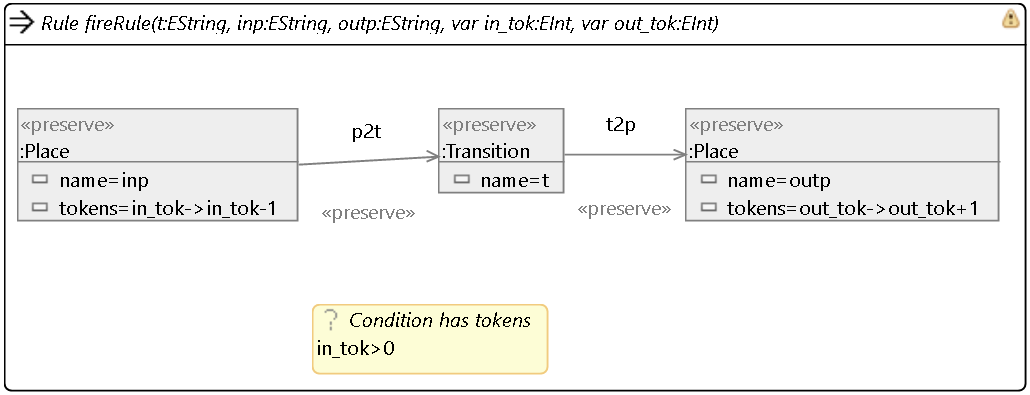
\includegraphics[width=0.8\textwidth]{images/firetransition.png}
\caption{A transition can fire if there is at least a single token in the source place}
\label{fig:firerule}
\end{figure}

There is only a single rule \textit{fireRule} as shown in Fig.~\ref{fig:firerule} which allows to move a single token from a place to another place. 
As usual for MoMOT, the parameters of the rule uniquely identify the rule match. Even though the model is simple, the number of models generated
by applying this rule multiple times can be huge, especially if multiple tokens are used.

\paragraph{Object-oriented refactoring}

This example~\footnote{Also see \url{http://martin-fleck.github.io/momot/casestudy/class_restructuring/} for a detailed description}, which was initially taken from the TTC 2013, contains entities with named, typed properties and generalizations. 
Originally, it was used as optimization problem to reduce the number of attributes and entities in a system. However, in this paper
we want to find a way to refactor a system in a particular fashion. The three refactoring rules are (a) Pull up attribute, which moves an attribute existing in all subclasses into the superclass, (b) extract super class, which creates a new superclass if an attribute is existing in some, but not all subclasses of a particular class, or (c) create root class, which is the same if the classes do not have any existing superclass.

In contrast to both examples above, this example changes the model structure by adding entities and generalizations and removing properties.



\subsection{Analysis}

In the following, we describe the results of the experiments conducted in terms of the research questions.


While many general distance metrics exists, we opted for an EMF-compare based one as this tool is widely used for differentiating models. In particular, we calculate the difference between two models by counting the percentage of model differences in the whole model.

Initially, we generated 100 examples of pairs of source and target model for each case. As the results for the Refactoring case initially were good, but not statistically significant, we generated 1000 examples for this case as well. While the source model was generated randomly within
certain predefiend parameters, the target model was generated by randomly applying transformations to the source model. 
However, for the Pacman case, we had to add more "`intelligent"' rules to generate sensible target states as typically, randomly applying move operations
just lead to Pacman being killed soon by running into a ghost or just being eaten by a ghost. Here, the rules force Pacman to eat neighboring food when possible and avoiding any ghosts. The search process itself does not use these rules, but just the generic ones.

For each example, only a single run was conducted. Then, the final solutions generated by each run were compared.
A solution is considered better if the number of transformations used to reach the target model is smaller. If a run did 
not produce any transformation sequences matching the target model, this number is considered to be infinite. We did not consider cases where 
the result models were not exactly matching the target model as at least two different distance metrics could be used for that.

To determine which fitness function was better we assumed that if both fitness functions would produce equal results,
there was a 50/50 chance that either fitness function was better for runs which produced differences.
For each example, we calculated the chance that the distance metrics would be as good or better just by chance.
Thus, we can reject the null hypothesis that the domain specific fitness function is not better if this value is below 5\%.

%Values are so low - calculate p exactly!


\subsubsection{Results for RQ1 Search Space Exploration}

\begin{table}
\begin{tabular}{|c|c|c|c|c|}
\hline
 & Generic & Equal & Domain-specific & p-value \\
\hline
Pacman & 1 & 73 & 27 & \textbf{.11E-7} \\
\hline
Petrinet & 26 & 30 & 45 & \textbf{.016} \\
\hline
Refactor (100) & 22 & 47 & 32 & .11 \\
\hline
Refactor (1000) & & & & \\
\hline
\end{tabular}
\label{tab:resultsrq1}
\end{table}

Table~\ref{tab:resultsrq1} shows the differences in the results quality for both approaches. For the Pacman case, we generated 8x8 fields with one Pacman, three ghosts, and 15 food, where all food and all other entities were randomly distributed. The Petrinet case used 10 places and 1 to 2 transitions per place and 1 to 2 outgoing place per transition. Also, the net was initialized with between 2 and 4 tokens. The Refactor case used 6 entities, 1 to 5 attributes per entity, where each name was one of 8 possible names and each attribute name was associated to 1 to 3 types. Also, each entity had a 50\% chance to have a random superclass. 

The Pacman case was rather hard for both fitness functions - all the equal values are due to no solution being found in either case. However, in this instance the domain specific fitness function could show its benefits, as it could solve the problem in 27 cases, while the generic one could only solve it in one case, yielding a significant difference. In contrast, the Petrinet case was rather easy for both algorithms, as most of the equal values were due to both algorithms finding solutions having the exact same quality. Still, the domain specific fitness function allowed us was at least statistically significantly better.


\subsubsection{Results for RQ2 Search Time}

We determined the rate of convergence by storing the solutions found after each evaluation step



%* Linearize quality to make comparable
% - Alternative: Just make "`normal"' comparison in each step?

%* Calculate average solution quality over the course of the runs
% - Save solutions after each step
% - Maybe different distance function implement? Normalize with initial difference
% - Just show it, values ... I am not sure that they would be sensible here

While exact time measurements were not taken, the domain-specific distance function always was faster, sometimes drastically faster,
than the generic EMF-compare based one. 

%- Time: EMFCompare takes longer (difficult to measure reliable, as performance VS solution quality metrics collide)
%- Unexpected: EMFCompare converges faster initially for many models - why?
% * Distance metrics used is EMFCompare ...

\subsection{Threats to validity}

\subsection{Discussion}
The current implementation assumes that M1 and M2 have the same position objects (none are deleted or created). This is too restrictive. Therefore M1 and M2 should be preprocessed by merging their position elements and then use the move distance. One possibility is to use EMFCompare to merge M1 and M2 based on the position elements.

Interestingly, when you run the Pacman test with models/input12missing.xmi and models/targetNoPac.xmi in one signle run, you don't necessarily get always the same sequence of rule applications. That is because p1 can be killed anywhere along the path of g1. 

\section{RELATED WORK}
With respect to the contribution of this paper, we discuss two threads of related work. First, we discuss approaches for model differencing. Second, we discuss approaches which cluster models based on distance metrics in the context of analysing model repositories.

\subsection{Model Differencing} In the last decade, there have been many works published for deriving model differences which are based on atomic operations, e.g., see~\cite{} for concrete approaches and~\cite{} for surveys. In~\cite{} an approach is presented to derive a domain-specific difference language for atomic changes for a particular metamodel.
 To the best of our knowledge, these approaches are not supporting the computation of distances as we propose in this paper.
In addition to these approaches focusing on atomic operations, there have been also some works published on the detection of domain-specific operations. For instance, Xing and Stroulia [10] present an approach for detecting refactorings in evolving software models which is integrated in UMLDiff. Refactorings
are expressed by change pattern queries used to search a
difference model obtained by a state-based model comparison.
The approach by Vermolen et al. [11] copes with the detection
of complex evolution steps between different versions of a
metamodel to allow for a higher automation in model
migration. They use a diff model comprising primitive changes
as input and calculate, on this basis, complex changes. The
approach is tailored to the core of object-oriented
metamodeling languages, but follows a similar methodology as
UMLDiff. However, a specific feature is the detection of so-called
masked changes, i.e., changes, which are hidden by other
changes in a way that their effect is partially or also totally
missing in the revised model, by defining additional detection
rules. Furthermore, there is the work of Küster et al. [12] for
calculating hierarchical change logs including compound
changes in the absence of recorded change logs. The authors
apply the concept of Single-Entry-Single-Exit fragments to
calculate the hierarchical change logs after computing the
correspondences between two process models. Thereby,
several atomic changes are hidden behind one compound
change. The use of graph transformations to collect atomic
changes on models into more meaningful changes called user-level
changes has been reported in [13].

In~\cite{} we have presented an domain-specific operation detection approach which transforms model transformation rules into diff patterns which can be matched on diff models. In follow-up work, we presented the first search-based approach for detection operation sequences between two model versions without requiring a diff model as basis to detect operations. However, we resorted on atomic diff models in the fitness function to compute how close a computed model is with respect to the given revised model. 

To sum up, many approaches have been proposed to compute difference models in the past. However, to the best of our knowledge, none focussed on distances as we present in this paper. Also the comparison of using differences or distances for searching for operation sequences is a novel contribution of this paper. 

\subsection{Model Clustering}

Recent work discusses dedicated support to cluster models in model repositories~\cite{}. Thus the setting is different to the two-way or three-way comparison of models which is mostly studied in the model comparison and model versioning fields. In such cases, it is assumed that many models have to be compared at once. Thus, a generic clustering technique for models is proposed which is based on the translation of model to a vector space model. Based on this vector space representation, clustering distance measures can be reused such as Manhattan distance.

\url{http://ceur-ws.org/Vol-2245/ammore_paper\_2.pdf}

\url{http://www.scitepress.org/DigitalLibrary/Link.aspx?doi=10.5220\%2f0005799103610367}



\section{CONCLUSION}
Summary


Conclusions


Future work 

Our approach may be used for model synchronization. 

\bibliographystyle{alphaurl}
\bibliography{biblio}

\end{document}
